\chapter{Evaluation}
\label{ch:evaluation}

This chapter evaluates the efficacy of the TCM-Sage system compared to a non-specialized large language model (LLM) baseline. The evaluation is conducted through a blind A/B testing framework, the "Arena," involving practitioners and students from the Traditional Chinese Medicine (TCM) community.

\section{Experimental Setup}

The evaluation framework was designed to isolate the impact of the specialized RAG (Retrieval-Augmented Generation) pipeline and the TCM-specific system prompt.

\subsection{System Configurations}
Two distinct system configurations were compared:
\begin{enumerate}
    \item \textbf{Treatment (TCM-Sage):} The full pipeline described in Chapter 4, including specialized RAG context from 17 classical texts, SymMap v2.0 knowledge graph integration, and the professional TCM system prompt.
    \item \textbf{Baseline (Plain LLM):} A generic configuration using the same underlying Qwen model but with a "helpful assistant" prompt. To simulate a modern AI's capabilities, the baseline had access to \textbf{DuckDuckGo Web Search} (5 results), representing the current standard for general-purpose retrieval.
\end{enumerate}

\subsection{Blind A/B Design}
A total of 59 votes were collected from a pool of TCM students and practitioners. The evaluation used a blind design:
\begin{itemize}
    \item \textbf{Randomization:} The positions of the Treatment and Baseline responses (A/B) were randomized for each query.
    \item \textbf{Interaction:} Voters entered a clinical or theoretical query and received two simultaneous streams.
    \item \textbf{Metrics:} After reading both responses, voters could select "A is Better," "B is Better," or "Tie." Votes were stored in a JSONL format for statistical analysis.
\end{itemize}

\section{Quantitative Results}

The primary goal of the quantitative analysis was to determine if the TCM-Sage system provided a statistically significant improvement over a general-purpose LLM.

\subsection{Comparative Performance}
The distribution of the 59 votes is summarized below:
\begin{itemize}
    \item \textbf{TCM-Sage Wins:} 38 (64.4\%)
    \item \textbf{Plain LLM Wins:} 15 (25.4\%)
    \item \textbf{Ties:} 6 (10.2\%)
\end{itemize}

The TCM-Sage system outperformed the baseline in over 60\% of cases, more than doubling the win rate of the general-purpose search-augmented model.

\begin{figure}[H]
\centering
\begin{minipage}{0.48\textwidth}
    \centering
    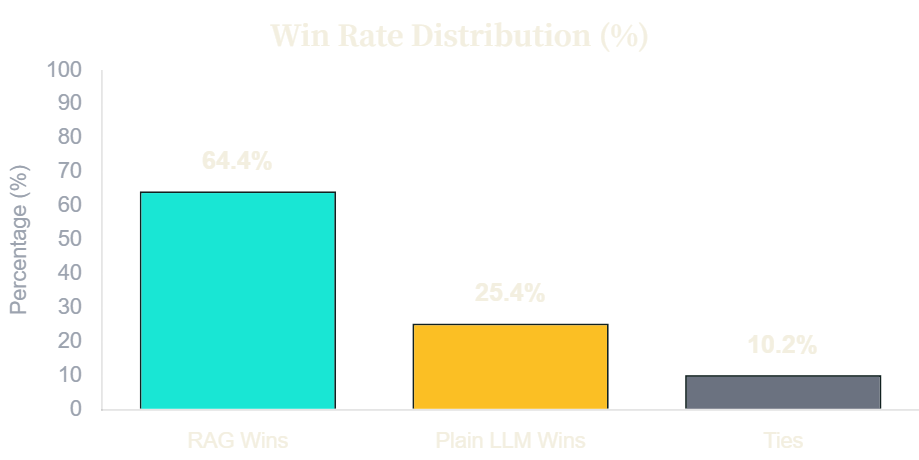
\includegraphics[width=\textwidth]{figures/arena-win-rate.png}
    \caption{Win rate distribution across the three outcomes.}
    \label{fig:winrate}
\end{minipage}\hfill
\begin{minipage}{0.48\textwidth}
    \centering
    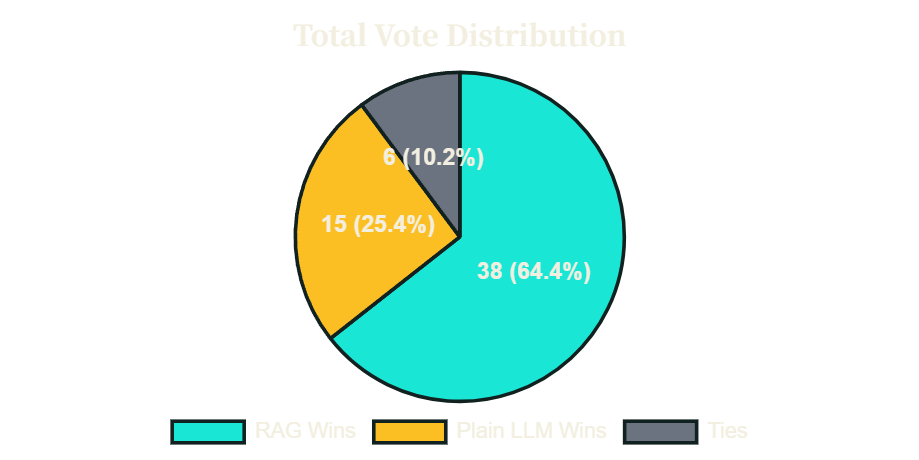
\includegraphics[width=\textwidth]{figures/arena-vote-distribution.png}
    \caption{Total vote distribution (N=59).}
    \label{fig:votedist}
\end{minipage}
\end{figure}

\subsection{Statistical Significance}
To rigorously test the null hypothesis that there is no difference between the two systems, a \textbf{paired t-test} was performed. Each vote was encoded as a paired score: 1 for a TCM-Sage win and 0 for a Plain LLM win (with ties encoded as 0.5 for both). The test evaluated whether the mean paired difference between RAG and plain scores was significantly different from zero.
\begin{itemize}
    \item \textbf{t-statistic:} 3.44
    \item \textbf{p-value:} 0.0011
\end{itemize}
With $p < 0.01$, the results are highly significant, allowing us to reject the null hypothesis.

\subsection{Effect Size}
\textbf{Cohen's d} was calculated to measure the magnitude of the improvement:
\begin{itemize}
    \item \textbf{Cohen's d:} 0.45
\end{itemize}
An effect size of 0.45 indicates a \textit{medium effect}, suggesting that while the general-purpose model is a capable baseline, the specialized TCM-Sage system provides a meaningful and consistent advantage in the quality of clinical reasoning and source accuracy.

\section{Temporal Analysis}

The evaluation was conducted over a four-day period (April 3 to April 6, 2026), during which the system underwent minor iterative refinements based on initial feedback.

\begin{itemize}
    \item \textbf{April 3:} 2 RAG / 1 Plain / 0 Ties (3 votes) --- Initial testing phase.
    \item \textbf{April 4:} 13 RAG / 8 Plain / 6 Ties (27 votes) --- Main testing batch from student groups.
    \item \textbf{April 5:} 8 RAG / 0 Plain / 0 Ties (8 votes) --- Post system prompt and retrieval improvements.
    \item \textbf{April 6:} 12 RAG / 6 Plain / 0 Ties (18 votes) --- Extended testing with a wider group of practitioners.
    \item \textbf{April 7:} 3 RAG / 0 Plain / 0 Ties (3 votes) --- Continued testing.
\end{itemize}

The cumulative trend shows a consistent preference for TCM-Sage, with a notable peak in performance after specific clinical knowledge (e.g., unit conversions) was hard-coded into the system prompt.

\section{Qualitative Feedback and Case Studies}

Qualitative feedback from TCM professionals provided deeper insights into the specific strengths and weaknesses of both systems.

\subsection{Dosage and Unit Conversion}
A doctoral student at Guangzhou University of Chinese Medicine, who also practices at the Guangdong Provincial Hospital of TCM, tested a query regarding the dosage of \textit{Mahuang Tang}. He observed that the general LLM (Baseline), aided by its web search capability, correctly identified the modern unit conversion for Han Dynasty weights. By contrast, the TCM-Sage system at that time provided an incorrect conversion (1 \textit{liang} $\approx$ 3g instead of $\approx$ 13.8g), because the classical texts in the knowledge base do not contain modern unit conversion data.

\textit{Outcome:} This feedback led to the immediate implementation of the \textit{Measurement Conversion} table (1 \textit{liang} $\approx$ 13.8g) in the system prompt. Subsequent tests showed that practitioners found the corrected system far superior to the baseline, as it provided both historical accuracy and modern relevance.

\subsection{Source Traceability}
Students consistently highlighted the \textbf{Citation Panel} as the most valuable feature. One student noted: "The ability to see the original classical text immediately, without having to copy-paste the formula name into a search engine to verify the source, is the key value of this system." This indicates that the \textit{traceability} provided by RAG is as important as the \textit{content} of the generated response.

\subsection{Diagnostic Hedging and Safety}
A doctoral student who also practices as a physician noted that the early version of the system was ``over-assertive'' in its diagnosis of \textit{Pi Xu} (Spleen Deficiency) based on limited symptoms. Following this, \textbf{Hedging Principles} were added to the prompt, requiring the system to use more tentative language (``The symptoms suggest a possibility of...'') when data is incomplete. The practitioner later confirmed that the updated responses felt more like a professional consultation than a ``black-box'' diagnosis.

\subsection{Novel Clinical Insights}
In one recorded case, a student consulted the system for a sore throat. The system suggested \textit{Jiegeng Tang}, a classical formula the student had not considered. Upon reviewing the provided citations, the student confirmed the validity of the recommendation. This demonstrates the system's potential as a "clinical co-pilot" that can surface relevant but overlooked classical knowledge.

\section{Limitations of Evaluation}

While the results are statistically significant, several limitations must be acknowledged:
\begin{enumerate}
    \item \textbf{Sample Size:} 59 votes are sufficient for statistical significance but do not represent a comprehensive clinical trial.
    \item \textbf{Voter Demographic:} The majority of voters were TCM students rather than senior clinicians with decades of experience.
    \item \textbf{Evaluation Format:} The Arena tests overall user preference, which includes factors like formatting and tone, not just clinical accuracy.
    \item \textbf{Prompt Influence:} Because the system prompts differed between the two models, the evaluation measures the effectiveness of the \textit{entire pipeline} (Prompt + RAG + KG), not just the retrieval component in isolation.
\end{enumerate}

\section{Discussion of Results}

The results of the evaluation demonstrate that a specialized RAG system tailored for TCM significantly outperforms a general-purpose search-augmented LLM.

\begin{itemize}
    \item \textbf{Accuracy vs. Verifiability:} The primary advantage of TCM-Sage lies in its ability to provide verbatim classical citations. While the general LLM can often ``summarize'' TCM knowledge from the web, it frequently hallucinates formula origins or misinterprets classical syntax.
    \item \textbf{The Value of Domain Knowledge:} The integration of a specialized knowledge graph and a professional system prompt (including ancient-to-modern measurement conversions) is essential for clinical utility. Without these, even a high-quality RAG system is prone to fundamental errors in interpretation.
    \item \textbf{Impact on the Field:} The $p = 0.0011$ result strongly suggests that specialized AI tools can provide a higher standard of information for the TCM community than general-purpose assistants, particularly in the areas of citation traceability and classical methodology adherence.
\end{itemize}
